%-------------------------------------------------------------------------
%-------------------------------------------------------------------------
%-------------------------------------------------------------------------
%\begin{figure*}
%\centering
%\vspace{-0.25in}
%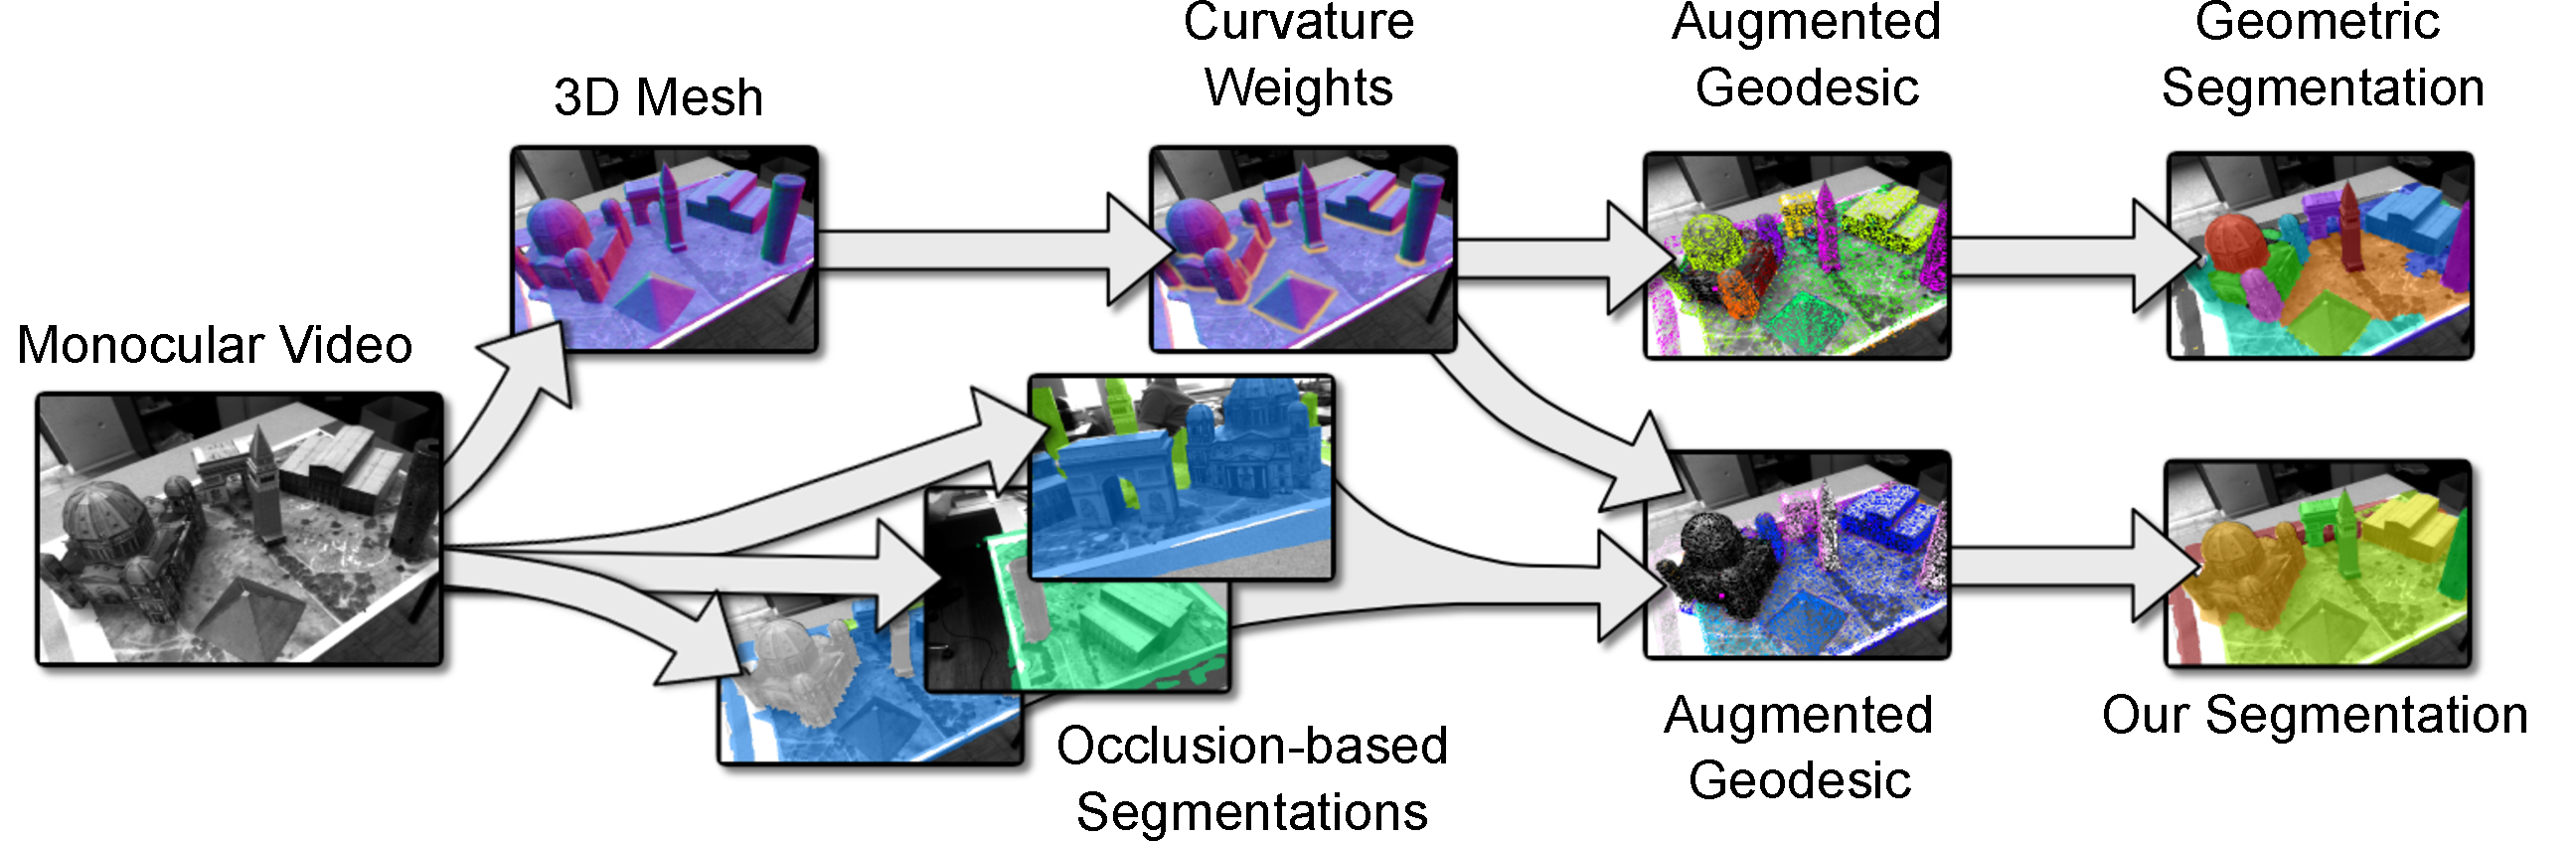
\includegraphics[height=2.25in]{../figs/pipeline.pdf}
%\captionof{figure}{Viewpoint-adaptive segmentation pipeline \TODO{Make this figure work right underneath the title if possible}}\label{fig:pipeline}
%\vspace{-0.25in}
%\end{figure*}

\iffalse
\begin{abstract}
  We describe a method to segment a static three-dimensional scene using monocular video. The result
is a dense reconstruction of three-dimensional geometry, partitioned into connected components with
consistent geometric and topological characteristics as seen from the viewer. This is made possible
by a number of technical advances to define and compute an adaptive geodesic distance on the scene,
which incorporates its geometry, topology, and photometry. This partitioning is explicitly viewpoint-dependent,
with segments being created based on the relevant portions of the scene implicit in the changes of viewpoint through the video.
 We also introduce a new ground-truthed dataset to evaluate our approach in
 comparison with standard approaches to segmenting
dense geometry.
\end{abstract}
\fi

%-------------------------------------------------------------------------
%-------------------------------------------------------------------------
%-------------------------------------------------------------------------
\section{Introduction}
\iffalse
\TODO{re: no kinect? argument about ubiquity of monocular video w/ phones?}
\TODO{Abstract/Intro should motivate robot vision/segmentation for interaction to sound more appropriate for RSS}

a method to endow a scene, densely reconstructed from monocular video, with a metric that incorporates image topology, namely occlusions.
Occlusions inform the granularity of the segmentation. OF all possible scene segmentations, those that do not trigger occlusions in response to viewer motion are neglected.
Occlusions inform the level of granularity of teh segmentation of the scene. However, segmenting the images and back-projecting the result onto tye scene does not yield temporally consistent (viewpoint-independent) results, thus we develop ….
\fi

In this chapter, we present a method, illustrated in Fig. \ref{fig:pipeline}, to endow a scene, densely reconstructed from monocular video, 
with a metric that incorporates geometric homogeneity and image topology through occlusions. While the latter are temporally inconsistent (they change with the
video), the way they change is spatially consistent, an observation key to defining affinities that allow us to partition the scene into coherent ``objects'' at a level of granularity relevant to the viewer. Occlusions inform the scale of the segmentation, allowing the selection of a partitioning of the scene, out of all possible partitions, that respects the occlusions present in the video. For robotic interaction tasks, such as manipulation or obstacle avoidance, the granularity of the scene representation can be critical, and our approach focuses the scene segmentation task on objects that generate occlusions in the images due the motion of the viewer relative to the scene.  

To achieve this, we employ a robust metric on the scene using a combination of curvature-based geodesics on a 3D mesh and back-projected occlusion-constrained image segmentations. The spatial consistency of these segmentations on the scene allows our segmentation method to adapt to the scale informed by the occlusions in the video. While one could employ trained object detectors at the outset to arrive at a semantic segmentation of the scene, we focus on low-level geometric and topological cues
first, to segment the scene and images into coherent regions, where one could then deploy object detectors if so desired. Semantic analysis of the scene involves object identities and relations, and knowledge
of scene geometry, topology, and putative object regions are key to infer the latter. This is the focus of our work.

The remainder of the chapter is organized as follows: In Sec. \ref{sec:sceneModel} we formulate scene (and video) segmentation as a selection problem on the set of potential nested partitions of the underlying scene based on homogeneity properties, and Sec. \ref{sec:signatures} presents occlusion-based image segmentation as a scale-selection mechanism on this set of potential partitions. Sec. \ref{sec:curvGeod} 
presents the construction of a curvature-augmented geometry on a 3D mesh used in Sec. \ref{sec:adaptiveGeo} to regularize these occlusion-based 
selections obtained from the image frames through an adaptive geodesic 
that combines these two components to perform a scene segmentation at the level of granularity relevant to the viewer. Finally, Sec. \ref{sec:evaluation} shows a quantitative and qualitative evaluation of our scale-adaptive segmentation scheme on a ground-truthed dataset of monocular dense reconstructions that we have collected. 

The work described here is the result of a fifty-fifty collaboration with Konstantine Tsotsos, who designed and assembled the 3D pipeline, made significant contributions to the 
``object distance'' metric, and implemented the segmentation scheme.
\iffalse
\TODO{There is a lack of details and motivation for the geodesic distance function, Sec. 2.4. This is regrettable, since this is the main novelty of the approach. The rest of the paper feels like a combination of other prior work, and not so much novel information is presented.}
\fi
%-------------------------------------------------------------------------
\subsection{Contributions and Related Work}
There is a vast body of literature pertaining to semantic segmentation of {\em images}
\cite{VittorioFerrari:2006uf,AlexanderVezhnevets:2012tw,Martnez:2004dz,WeiFeng:cw,GuofengZhang:jma,
ulen-strandmark-etal-itmi-12,Russell06,ics_nips11,Lempitsky11,Kumar10,nieuwenhuis-et-al-ijcv12};
our work is particularly related to {\em joint} segmentation (a.k.a. ``co-segmentation'') of
multiple images, or {\em video}
\cite{vezhneva:2012tb,GuofengZhang:jmb,Cremers-et-al-11,Schoenemann-Cremers-pami10,lezama11,
carreira_eccv12}. However, the goal of such
approaches is a partitioning of the spatio-temporal
image volume, not of the {\em scene} that generated it. Seeking a segmentation of the scene allows
us to bypass the complex and discontinuous changes in the partitioning of the video due to scale,
spatial quantization, and occlusions.  Furthermore, occlusions provide local ordering constraints that can be
used to partition the image into
``layers'' \cite{wangA94,Reid:2010ca,GuofengZhang:jm,Cremers-12,Kumar08,Kumar05a} by solving a
convex optimization problem \cite{Cremers-et-al-11}. In all of these cases, ``objects'' are
collections of pixels that are often {\em temporally inconsistent} as the local ordering constraints
can change over time (think of a merry go round), producing flickering segmentations. However, by
by using occlusions as topological cues these segmentations tend to correspond to spatially
consistent regions on the scene, even if their image labels are not temporally consistent. Our
method relies heavily on this observation to accumulate data-driven cues for the extent of
individual objects in the scene.

Our work can be interpreted as an attempt to combine multiple image segmentations (which depend on
both the scene and the viewer) into one persistent segmentation of the scene independent of the
viewer.  Since our method involves the intermediate reconstruction of a dense three-dimensional
model of the scene, which we do in real time, our work also relates to multiple-view stereo and
structure-from-motion, and in particular real-time dense multi-view
stereo \cite{davison,cremers,pock}. As an alternative, one could use an alternate range sensor
\cite{RobFergus:2012vh}, for instance based on structured light \cite{Newcombe2011a}, although
those perform poorly in natural illumination and have a fixed scale of interaction.

There are relatively few attempts to generate a dense label field in the {\em scene}
\cite{Kalogerakis:2010:labelMeshes}. While semantic labels have been attached to various forms of
3D reconstruction, these typically are {\em sparse} ({{\em e.g.,} collections of feature
descriptors and their coarse positions \cite{fei-fei,baoS12}).

Our work is also related to \cite{khler2013efficient}, in which Regression
and Decision Tree Fields are used to segment a 3D scene, and \cite{ren2012rgbd}, in which SVMs are used to
segment point clouds gathered from RGB-D data. Similarly, Bleyer et al.\ \cite{bleyerRR12} describe a 
method for labeling that is explicitly compatible with the 3D structure of the scene. Although
direct comparison with these algorithms is not possible as neither their code nor their datasets are
publicly available, in Sect.~\ref{sec:results} we report experiments on data similar in nature and
scale that we intend to release publicly upon completion of the anonymous review
process. Other related work includes
\cite{zhangJB11,stucklerBB12,atanasovSLKPD13}, where the focus is on manipulation. Additionally,
Zheng et al.\ \cite{zheng2013beyond} use 3D point clouds to find objects in
the scene using geometric and physical cues from RGB-D data. Most closely related to our
work are are the recent works of \cite{haene2013, slampp2013, sengupta2013, kundu2014}), all of
which generate semantic segmentations of the scene using responses from trained detectors as input.
We seek to generate segmentations at a similar level of abstraction (albeit without semantic
labels) through viewpoint-based topological homogeneity instead of semantic homogeneity (object detector responses). Our method
can also be thought of as a generic proposal scheme for regions within which to collect support for
semantic categorization based on geometric and viewpoint based contextual information.
Partitions based on solely geometric homogeneity have also been explored extensively by 
the 3D mesh segmentation community (\cite{Chen:2009:ABF, AZCXT11, lafarge2010}).

Our contributions are (a) a method for scene segmentation leveraging the spatial consistency of temporally
inconsistent image cues, (b) an adaptive geodesic distance function on the scene shaped by
spatially consistent image cues in the form of occlusions, (c) an object-level scene segmentation scheme that extends a real-time dense reconstruction system based on monocular video. To compare with standard
approaches for segmenting dense geometry, we have (d) collected a calibrated dataset with a variety
of objects of different scales and textures, indoor and outdoor, on natural and artificial
laboratory scenes. A key assumption for our dense monocular reconstruction pipeline is that the only
thing moving in the scene is the viewer. Extension beyond cases where this
assumption holds is desirable, but even the
static case is relevant to several applications from robotic inspection to autonomous navigation and
exploration.

